\chapter{Funktio}
Matematiikassa tutkitaan paljon asioiden välisiä riippuvuuksia. Tällaiset riippuvuudet voidaan muotoilla funktioiden avulla. Esimerkiksi tuotteen arvonlisäveroprosentti riippuu tuoteryhmästä. Tämä riippuvuus voidaan kirjoittaa funktiona eri tuotteiden joukolta $A$ reaalilukujen joukolle $\mathbb{R}$, missä funktio liittää jokaiseen tuotteeseen sen arvonlisäveroprosentin.


\laatikko{\emph{Funktiolla} $f(x)$ tarkoitetaan \emph{sääntöä}, joka liittää \emph{muuttujaan} $x$ arvon $y=f(x)$.}

\begin{esimerkki}
Määritellään funktio $f$ tavaroiden joukolta $A$ reaaliluvuille joka kuvaa jokaisen tavaran sen arvonlisäveroprosentille.
\[A = \{\text{ahvenfilee}, \text{AIV-rehu}, \text{auto}, \text{runokirja}, \text{ravintola-ateria}, \text{särkylääke}, \text{televisio}\}\]
[Selitys arvonlisäverokannoista ja $f(\text{ahvenfilee}) = 13$, $f(\text{AIV-rehu}) = 13$, $f(\text{auto}) = 23$, $f(\text{runokirja}) = 9$, $f(\text{ravintola-ateria}) = 13$, $f(\text{särkylääke}) = 9$, $f(\text{televisio}) = 23$]
\begin{center}
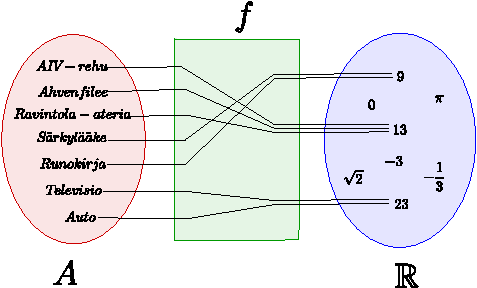
\includegraphics[width=13cm]{03-funktiot/kuvia/funktiokone-crop.pdf}
\end{center}
\end{esimerkki}

\laatikko{Funktio $f$ joukosta $A$ joukkoon $B$ on sääntö, joka liittää $A$:n jokaiseen alkioon $x$ täsmälleen yhden $B$:n alkion, jota merkitään $f(x)$. $A$:ta kutsutaan funktion $f$ määrittelyjoukoksi ja $B$:tä funktion $f$ maalijoukoksi.}

Käytäntöjä:
\begin{itemize}
\item $f(x) = y$ lausutaan: "Funktio saa arvon y pisteessä x."
\item Funktioita voidaan kutsua myös kuvauksiksi.
\item Funktion määrittely- ja maalijoukot jätetään usein merkitsemättä, jos ne ovat selviä asiayhteydestä. Tällä kurssilla maalijoukko on yleensä reaaliluvut.
\item Funktion sääntöä kutsutaan usein pelkästään funktioksi.
\end{itemize}

\begin{esimerkki}
Funktion argumentiksi eli funktion muuttujaksi kutsutaan sulkeiden sisällä olevaa osaa: esimerkiksi $f(x)$:ssä argumentti on $x$. Argumentti voi olla myös monimutkaisempi. Voimme kirjoittaa esim. $f(3x)$ tai $f(f(x))$.
\end{esimerkki}

\todo{lisää neliöjuuren määritelmä funktiona}

Funktion arvojoukko koostuu niistä maalijoukon alkioista, jotka funktio saa arvokseen ainakin yhdessä määrittelyjoukon pisteessä.

Funktion sääntö määritellään usein kaavan avulla. Voimme esimerkiksi määritellä funktion $f$ reaaliluvuilta reaaliluvuille kaavalla
\[f(x) = x^2 + 1,\]
eli $f$ liittää jokaiseen reaalilukuun $x$ luvun $x^2+1$. Tästä funktiosta huomaamme, että arvojoukko ei ole aina sama kuin maalijoukko. Esimerkiksi luku $0$ kuuluu funktion $f$ maalijoukkoon, mutta ei funktion $f$ arvojoukkoon, koska $x^2+1\geq 1$ neliön epänegatiivisuuden perusteella.

\missingfigure{kuva lähtöjoukoista ja maalijoukoista}

\esimerkki{Määritellään funktio $f$ kaavalla [kuva]
\[f(x) = \frac{1}{x-1}.\]
Funktiolle ei ole erikseen annettu määrittelyjoukkoa, joten se täytyy päätellä asiayhteydestä. Huomataan, että sääntö ei määrittele funktion $f$ arvoa kun $x = 1$, mutta kylläkin kaikilla $x\in\mathbb{R}\setminus\{1\}$ [vai?]. Näin ollen luonnollinen valinta määrittelyjoukoksi on $\mathbb{R}\setminus\{1\}$. Voimme myös selvittää funktion arvojoukon kiinnitettyämme määrittelyjoukon. Valitulla määrittelyjoukolla $\mathbb{R}\setminus\{1\}$ voimme muodostaa yhtälön $f(x)=a$ jollekin reaaliluvulle a. Tutkitaan, milloin tällä yhtälöllä on ratkaisu(ja).
\begin{align*}
a &= \frac{1}{x-1} & &| \, \text{Oletamme, että $x \neq 1$, jolloin voimme kertoa $(x-1)$:llä puolittain.} \\
a(x-1) &= 1 \\
x-1 &= \frac{1}{a} \\
x &= 1+\frac{1}{a} & &| \, \text{Huomaamme, että saamme ratkaisun kaikilla $a \neq 0$.} \\
& & &| \, \text{Yhtälö ei ole hyvinmääritelty, kun $a = 0$.}
\end{align*}
}
\begin{esimerkki}

jokin riippuu jostakin, esitä määrittely ja arvojoukko muodossa f:A->B
\end{esimerkki}

\todo{nollakohdan määritelmä ja löytäminen; kuvaajasta ja yhtälöstä}

Funktion nimeäminen, $f(x)$ (ei?) vastaa merkinnältään $\sin(x)$:ää. jälkimmäisen tunnistaa, tuttu funktio

\begin{tehtava}
Olkoon $f(x)=\frac{2^x+4}{x}$. Laske
\begin{enumerate}[a)]
\item $f(1)$
\item $f(2)$
\item $f(\frac{1}{2})$
\item $f(\frac{1}{3})$
\item $f(0)$
\item $f(-1)$
\end{enumerate}
\begin{vastaus}
\begin{enumerate}[a)]
\item $6$
\item $4$
\item $2\sqrt{2}+8$
\item $3\sqrt[3]{2}+12$
\item ei määritelty
\item $\frac{-9}{2}$
\end{enumerate}
\end{vastaus}
\end{tehtava}

% kai vaikeahko
\begin{tehtava}
Millä $x$:n arvoilla yhtälö $f(f(x)) = x$ pätee, kun
\begin{enumerate}[a)]
\item $f(x) = 1$
\item $f(x) = x$
\item $f(x) = x+1$
\item $f(x) = 2x$
\item $f(x) = 2x+1$?
\end{enumerate}
\begin{vastaus}
\begin{enumerate}[a)]
\item $x = 1$
\item kaikilla $x\in\mathbb{R}$
\item ei ratkaisuja
\item $x = 0$
\item $x = -1$
\end{enumerate}
\end{vastaus}
\end{tehtava}


\section{Usean muuttujan funktiot}

\laatikko{Funktiolla voi olla monta muuttujaa. Jos funktion $f$ arvo riippuu esimerkiksi muuttujista $x$ ja $y$, merkitään funktiota $f(x,y)$.}

\begin{esimerkki}

Olkoon suorakulmion korkeus $x$ ja leveys $y$. Tiedetään, että suorakulmion pinta-ala voidaan laskea kertomalla sen korkeus ja leveys keskenään, joten suorakulmion pinta-ala voidaan esittää tunnettujen pituuksien $x$ ja $y$ funktiona: $A(x,y)=xy$. Pituudet voivat olla vain positiivisia reaalilukuja, joten vaadimme, että $x>0$ ja $y>0$. Pinta-alaa esittää positiivinen reaaliluku, joten myös $A>0$. Kun tietyssä tapauksessa suorakulmion korkeus on 3 ja leveys 4, suorakulmion pinta-ala on $A(3,4)=3\cdot 4=12$ pinta-alayksikköä.

\end{esimerkki}




